% Ubah judul dan label berikut sesuai dengan yang diinginkan.
\section{Architecture}
\label{sec:architecture}

% Ubah paragraf-paragraf pada bagian ini sesuai dengan yang diinginkan.
\begin{figure}[hbtp] \centering
	% Nama dari file gambar yang diinputkan
	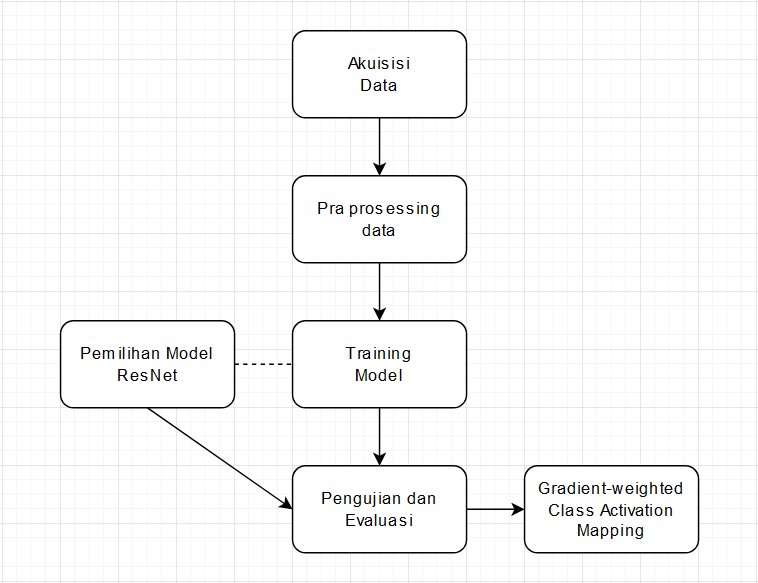
\includegraphics[scale=0.4]{gambar/diagramMethod.png}
	% Keterangan gambar yang diinputkan
	\caption{Methodology Diagram}
	% Label referensi dari gambar yang diinputkan
	\label{fig:diagramMethod}
\end{figure}

\subsection{Dataset}
\label{subsec:dataset}

The data utilized in this study were obtained from the Diabetic Retinopathy Analysis Grand Challenge, in the form of OCT-Angiography images.
A table, referenced as Table \ref{table:Datasettraining} in the text, provides a detailed overview of the data distribution utilized in this study.
\begin{figure}[hbtp]
	\centering
	\subfloat[\centering Non-DR]{{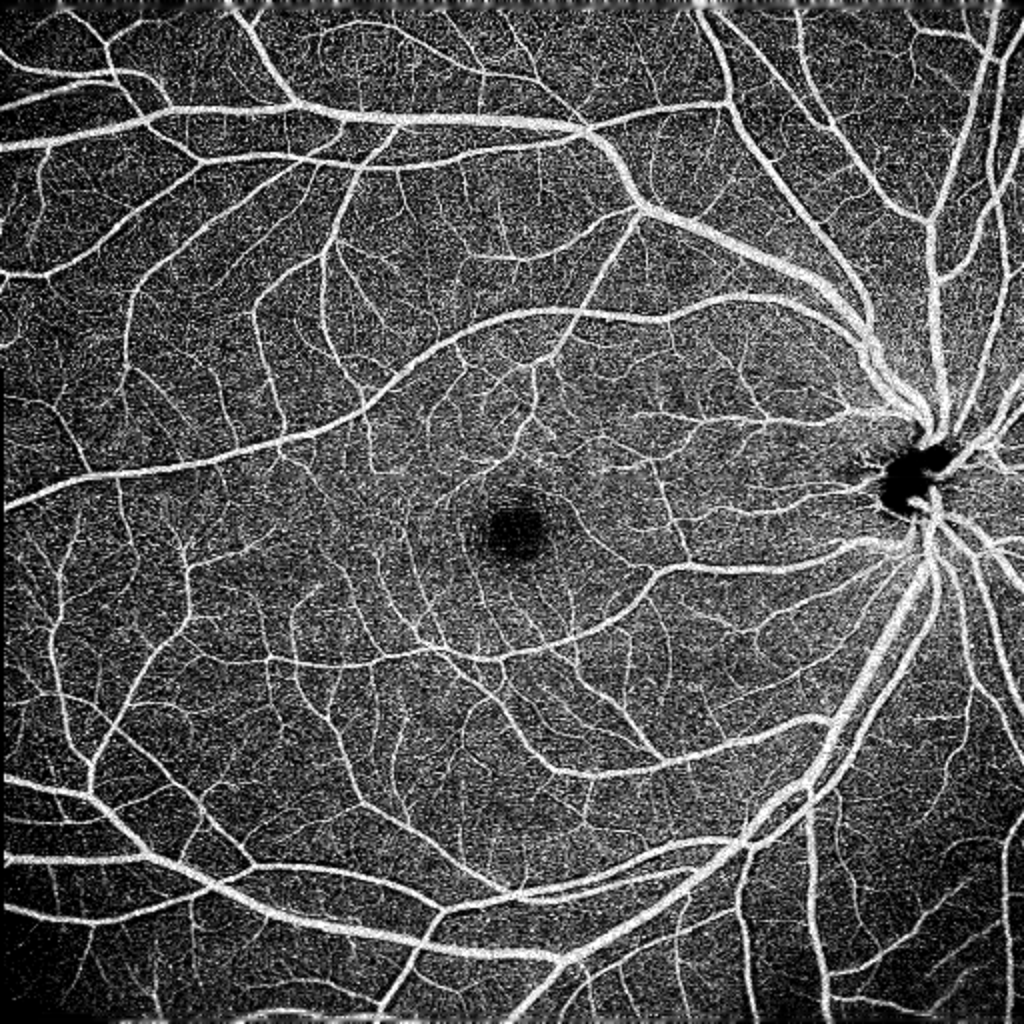
\includegraphics[width=2.5cm]{gambar/non-DR.png} }}%
	\subfloat[\centering NPDR]{{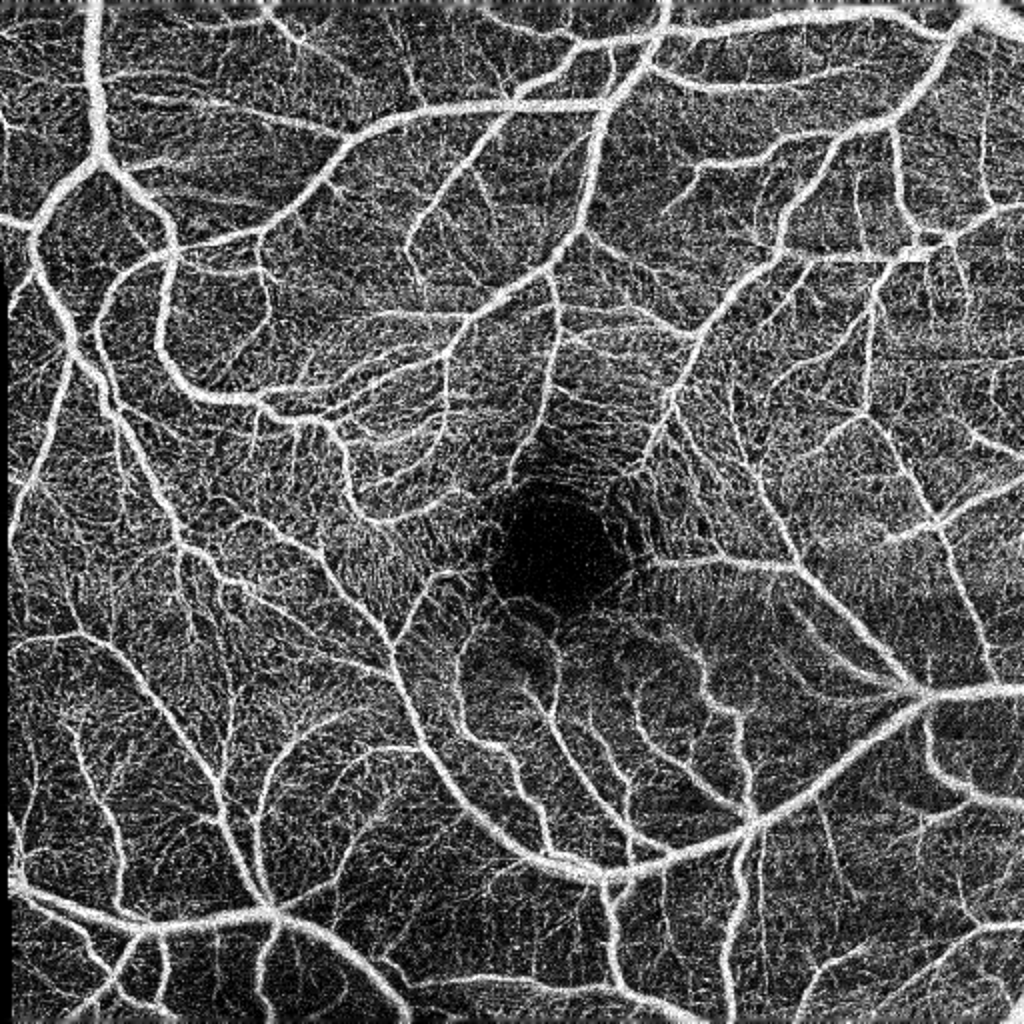
\includegraphics[width=2.5cm]{gambar/NPDR.png} }}%
	\subfloat[\centering PDR]{{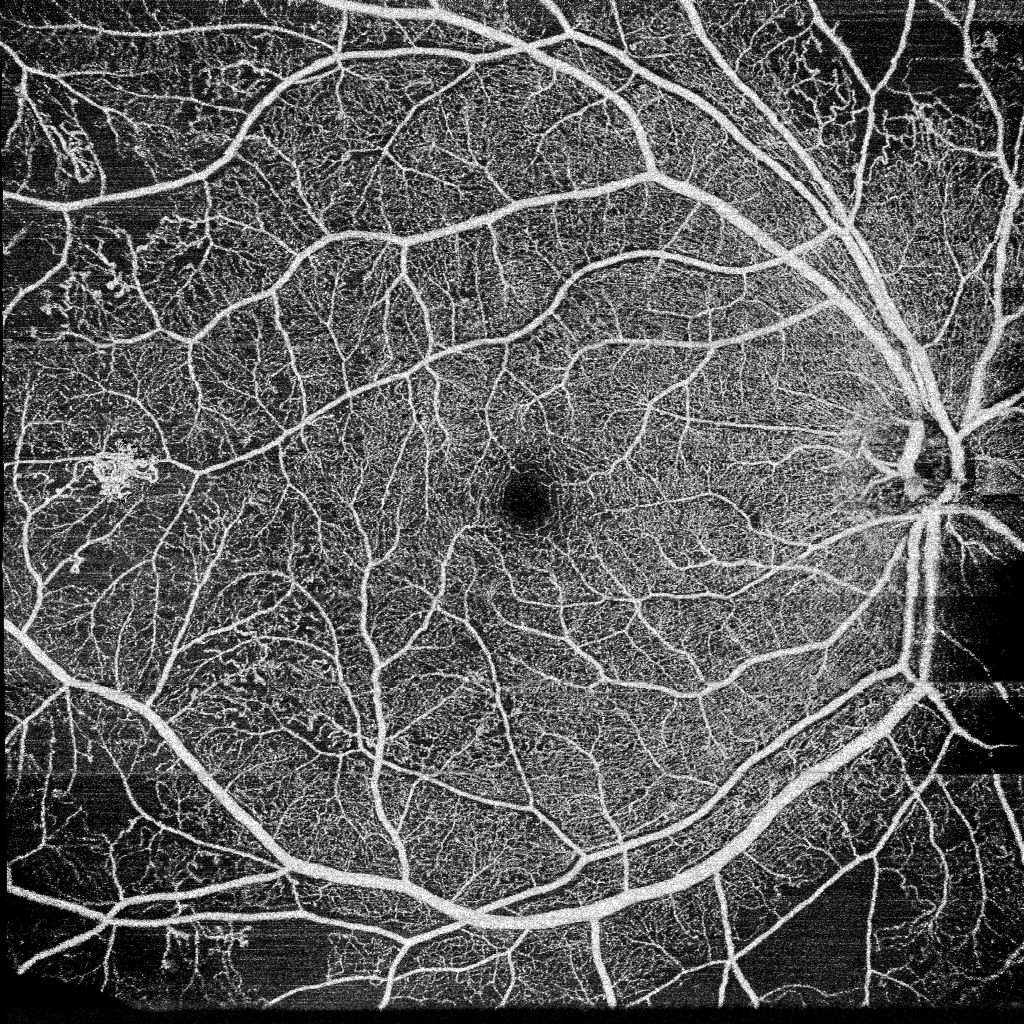
\includegraphics[width=2.5cm]{gambar/PDR.png} }}%
	\caption{Example of Fundus Images in the Dataset}
	\label{fig:sampleDataset}
\end{figure}

The image provided is a retinal fundus photograph, which is utilized for the evaluation of diabetic retinopathy. The image depicts the intricate details of the retinal vascular network, the optic disk, and the macular area. The following section provides a comprehensive account of the image in question.

Dataset Information from the DRAC Challenge
The dataset utilized for training and testing comprises the following:

	\begin{itemize}
		\item Training Set: 611 gambar
		\item Testing Set: 386 gambar
	\end{itemize}
Subsequently, the images in the training set are divided into two subsets, namely the training set and the validation set, with the number of images in each subset determined in accordance with the specifications outlined in Table \ref{table:Datasettraining}.
\begin{table}[hbtp]
	\begin{center}
	\caption{Table of distribution Set for Training and Validation}
	\label{table:Datasettraining}
	\begin{tabular}{|l|l|l|l|}
		\hline
		\rowcolor[HTML]{C0C0C0} 
		Label                                                & Classification & Amount & Total                                         \\ \hline
		\rowcolor[HTML]{FFFFFF} 
		\cellcolor[HTML]{FFFFFF}                             & non-DR      & 263    & \cellcolor[HTML]{FFFFFF}                      \\ \cline{2-3}
		\rowcolor[HTML]{FFFFFF} 
		\cellcolor[HTML]{FFFFFF}                             & NPDR        & 169    & \cellcolor[HTML]{FFFFFF}                      \\ \cline{2-3}
		\rowcolor[HTML]{FFFFFF} 
		\multirow{-3}{*}{\cellcolor[HTML]{FFFFFF}Training}   & PDR         & 56     & \multirow{-3}{*}{\cellcolor[HTML]{FFFFFF}488} \\ \hline
		\rowcolor[HTML]{FFFFFF} 
		\cellcolor[HTML]{FFFFFF}                             & non-DR      & 66     & \cellcolor[HTML]{FFFFFF}                      \\ \cline{2-3}
		\rowcolor[HTML]{FFFFFF} 
		\cellcolor[HTML]{FFFFFF}                             & NPDR        & 43     & \cellcolor[HTML]{FFFFFF}                      \\ \cline{2-3}
		\rowcolor[HTML]{FFFFFF} 
		\multirow{-3}{*}{\cellcolor[HTML]{FFFFFF}Validation} & PDR         & 14     & \multirow{-3}{*}{\cellcolor[HTML]{FFFFFF}123} \\ \hline
		\end{tabular}
	\end{center}
\end{table}

The images in the test set are employed to obtain an online assessment using the Quadratic Weighted Kappa metric, with the model from DRAC serving as a point of comparison. However, due to the absence of a label in the given test set, it is not feasible to utilize this set for the calculation of other metrics, such as precision, recall, and F1-score.

\subsection{Methodology}
\label{subsec:loremipsum}

The scenarios utilized for performance enhancement in ResNet model training are as follows. In this study, due to the limited dataset and the presence of unrepresentative classes, several methods were employed to achieve dataset balance.

\begin{itemize}
	\item Default
	
	No action was taken to balance the dataset. This method is performed for the control variable.
	
	\item Class-weight adjustment
	
	In this method, weight is added so that the underrepresented class has a higher weight.
\end{itemize}

\subsection{Model Training}
\label{sec:325}
The training of the model is conducted using the transfer learning method. The transfer learning method is performed using the ResNet model, which has been selected and trained with the ImageNet dataset.
The model architecture utilized is as described in \ref{subsec:loremipsum}, with the hyperparameters specified in Table \ref{tb:hyperParameterTraining}.
\begin{table}[hbtp]
	\begin{center}
		\caption{Hyperparameter}
		\label{tb:hyperParameterTraining}
		\begin{tabular}{|
		>{\columncolor[HTML]{C0C0C0}}l |l|lll}
		\cline{1-2}
		Input shape                                         & 224,224,3      &  &  &  \\ \cline{1-2}
		Opimizer                                            & Adam           &  &  &  \\ \cline{1-2}
		Loss Function                                       & Cross Entropy  &  &  &  \\ \cline{1-2}
		Learning Rate                                       & 0.1            &  &  &  \\ \cline{1-2}
		Momentum                                            & 0.9            &  &  &  \\ \cline{1-2}
		\cellcolor[HTML]{C0C0C0}                            & Step size = 10 &  &  &  \\ \cline{2-2}
		\multirow{-2}{*}{\cellcolor[HTML]{C0C0C0}Scheduler} & Gamma = 0.1    &  &  &  \\ \cline{1-2}
		Epoch                                               & 100            &  &  &  \\ \cline{1-2}
		Batch size                                          & 32             &  &  &  \\ \cline{1-2}
		\end{tabular}
	\end{center}
\end{table}

